The first section of this chapter covers the next major milestone, which is the thermal demonstrator. The next section gives an outlook for the \gls{STS}'s and the foreseen developments of the \gls{DCS}. Finally, the major achievements of the thesis will be highlighted and shortly described.

\section{Thermal Demonstrator}
Another important milestone toward the assembly of \gls{STS} is the thermal demonstrator. Its aim is to implement the dummy silicon sensor and electronics parts under realistic mechanical boundary conditions and to experimentally demonstrate the feasibility of \gls{STS}’s cooling concepts. 

Figure~\ref{fig:demo} depicts the thermal demonstrator with the respective dummy detector modules. These objects dissipate similar heat amount as the actual detector module. The excess heat has to be evacuated in order to prevent the silicon sensors from thermal runaway and reverse annealing. It should be achieved with a 3M 649 NOVEC based cooling system. The lowest temperature that the demonstrator will face, reaches down to \SI{-40}{\celsius}. 

\begin{figure}[!h]
    \centering
    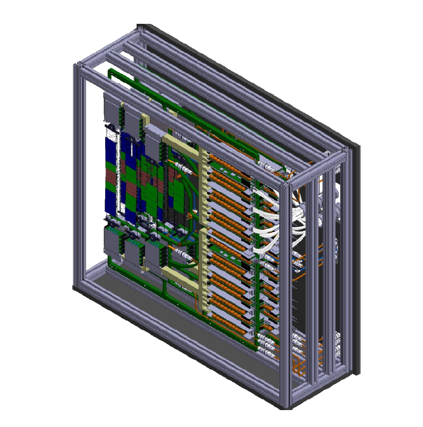
\includegraphics[width=0.65\columnwidth]{Chapter7/images/thermal_demo.png}
    \caption{CAD view of the thermal demonstrator~\cite{thermal_demo}. The dummy modules are mounted onto carbon ladders and placed in the C-frames, as the real silicon detectors will be.}
    \label{fig:demo}
\end{figure}
\label{demo}

 Due to the low temperatures inside the system, the frost point needs to be kept at values below \SI{-45}{\celsius}. To achieve this, a dedicated air drying system was developed and will be tested together with all the other services. 
 
 The thermal demonstrator serves not only to demonstrate and evaluate the cooling of\gls{STS} but also to perform long-term humidity and dew point measurements with the \gls{FOS} and sniffing system described in Chapter \ref{chap:fos}. The ambient conditions inside the demonstrator will reach similar ones as during \gls{STS} operation. Therefore, it's a unique opportunity to test the temperature, RH, and dew point sensors.
 
 Apart from the humidity sensors, the thermal demonstrator features also temperature sensors:
 \begin{itemize}
     \item to evaluate the performance of the cooling plate and the thermal interfaces, each dummy \gls{FEB} is populated with 3 temperature sensors,
     \item to assess how much heat should be dissipated by the dummy silicon sensors, there are also temperature sensors placed on each dummy.
 \end{itemize}

A few services including the cooling plant that delivers the cooling liquid to the test objects, humidity sensors but also interlocks, and control strategies can be developed and then adjusted for \gls{STS}. Hence, the thermal demonstrator is also a perfect opportunity to develop control system applications that will reduce the commissioning time of the \gls{STS}. In this case, further improvements of the containerized framework should be considered, e.g. orchestration\footnote{Orchestration is the coordination and management of computer systems, applications, and/or services.} of the containers. The next sections focus on the further improvements of the \gls{DCS} in order to have a reliable and easy-to-maintain solution for the final systems. 